\documentclass[useAMS, usenatbib, a4paper]{mnras}
\pdfsuppresswarningpagegroup=1

\usepackage[spanish,es-minimal,english]{babel}
\usepackage[utf8]{inputenc}
\usepackage{graphicx}
\graphicspath{ {../figs/} }
\usepackage{xcolor}
\usepackage{fixltx2e}
\usepackage{hyperref}
\usepackage{siunitx}
\usepackage{newtxtext}
\usepackage[varg,varvw,smallerops]{newtxmath}
\usepackage{booktabs}
\hypersetup{colorlinks=True, linkcolor=blue!50!black, citecolor=black,
  urlcolor=blue!50!black}
\usepackage{etoolbox}
\robustify\bfseries
\robustify\itshape
\bibliographystyle{mnras}

\sisetup{
  % explicit""+" is useful for velocities
  retain-explicit-plus = true,
  % prefer 10^6 over 1 x 10^6
  retain-unity-mantissa = false,
  % Use x +/- e instead of x(e)  
  separate-uncertainty = true,
  % Make sure to pick up bold font when used in section heading for instance
  detect-weight = true,
}
% A better \ion command that works in more circumstances
\newcommand\ION[2]{#1\,\scalebox{0.9}[0.8]{\uppercase{#2}}}
\newcounter{ionstage}
\renewcommand{\ion}[2]{\setcounter{ionstage}{#2}% 
  \ensuremath{\mathrm{#1\,\scriptstyle\Roman{ionstage}}}}
\newcommand\hii{\ion{H}{2}}
\newcommand\nii{[\ion{N}{2}]}
\newcommand\oiii{[\ion{O}{3}]}


\title{Kinematics of the Turtle Nebula (Will's part)}

\author[Henney]{
  William J. Henney\thanks{w.henney@irya.unam.mx}\\
  \foreignlanguage{spanish}{Instituto de Radioastronomía y
    Astrofísica, Universidad Nacional Autónoma de México, Apartado
    Postal 3-72, 58090 Morelia, Michaoacán, Mexico}
}
% These dates will be filled out by the publisher
\date{Accepted XXX. Received YYY; in original form ZZZ}

% Enter the current year, for the copyright statements etc.
\pubyear{2020}

\begin{document}
\label{firstpage}
\pagerange{\pageref{firstpage}--\pageref{lastpage}}
\maketitle

\begin{abstract}
  Material to be incorporated into the main paper by Teresa.
\end{abstract}
\begin{keywords}
  Atomic physics -- Radiative transfer -- Photodissociation regions
\end{keywords}


\begin{figure}
  \centering
  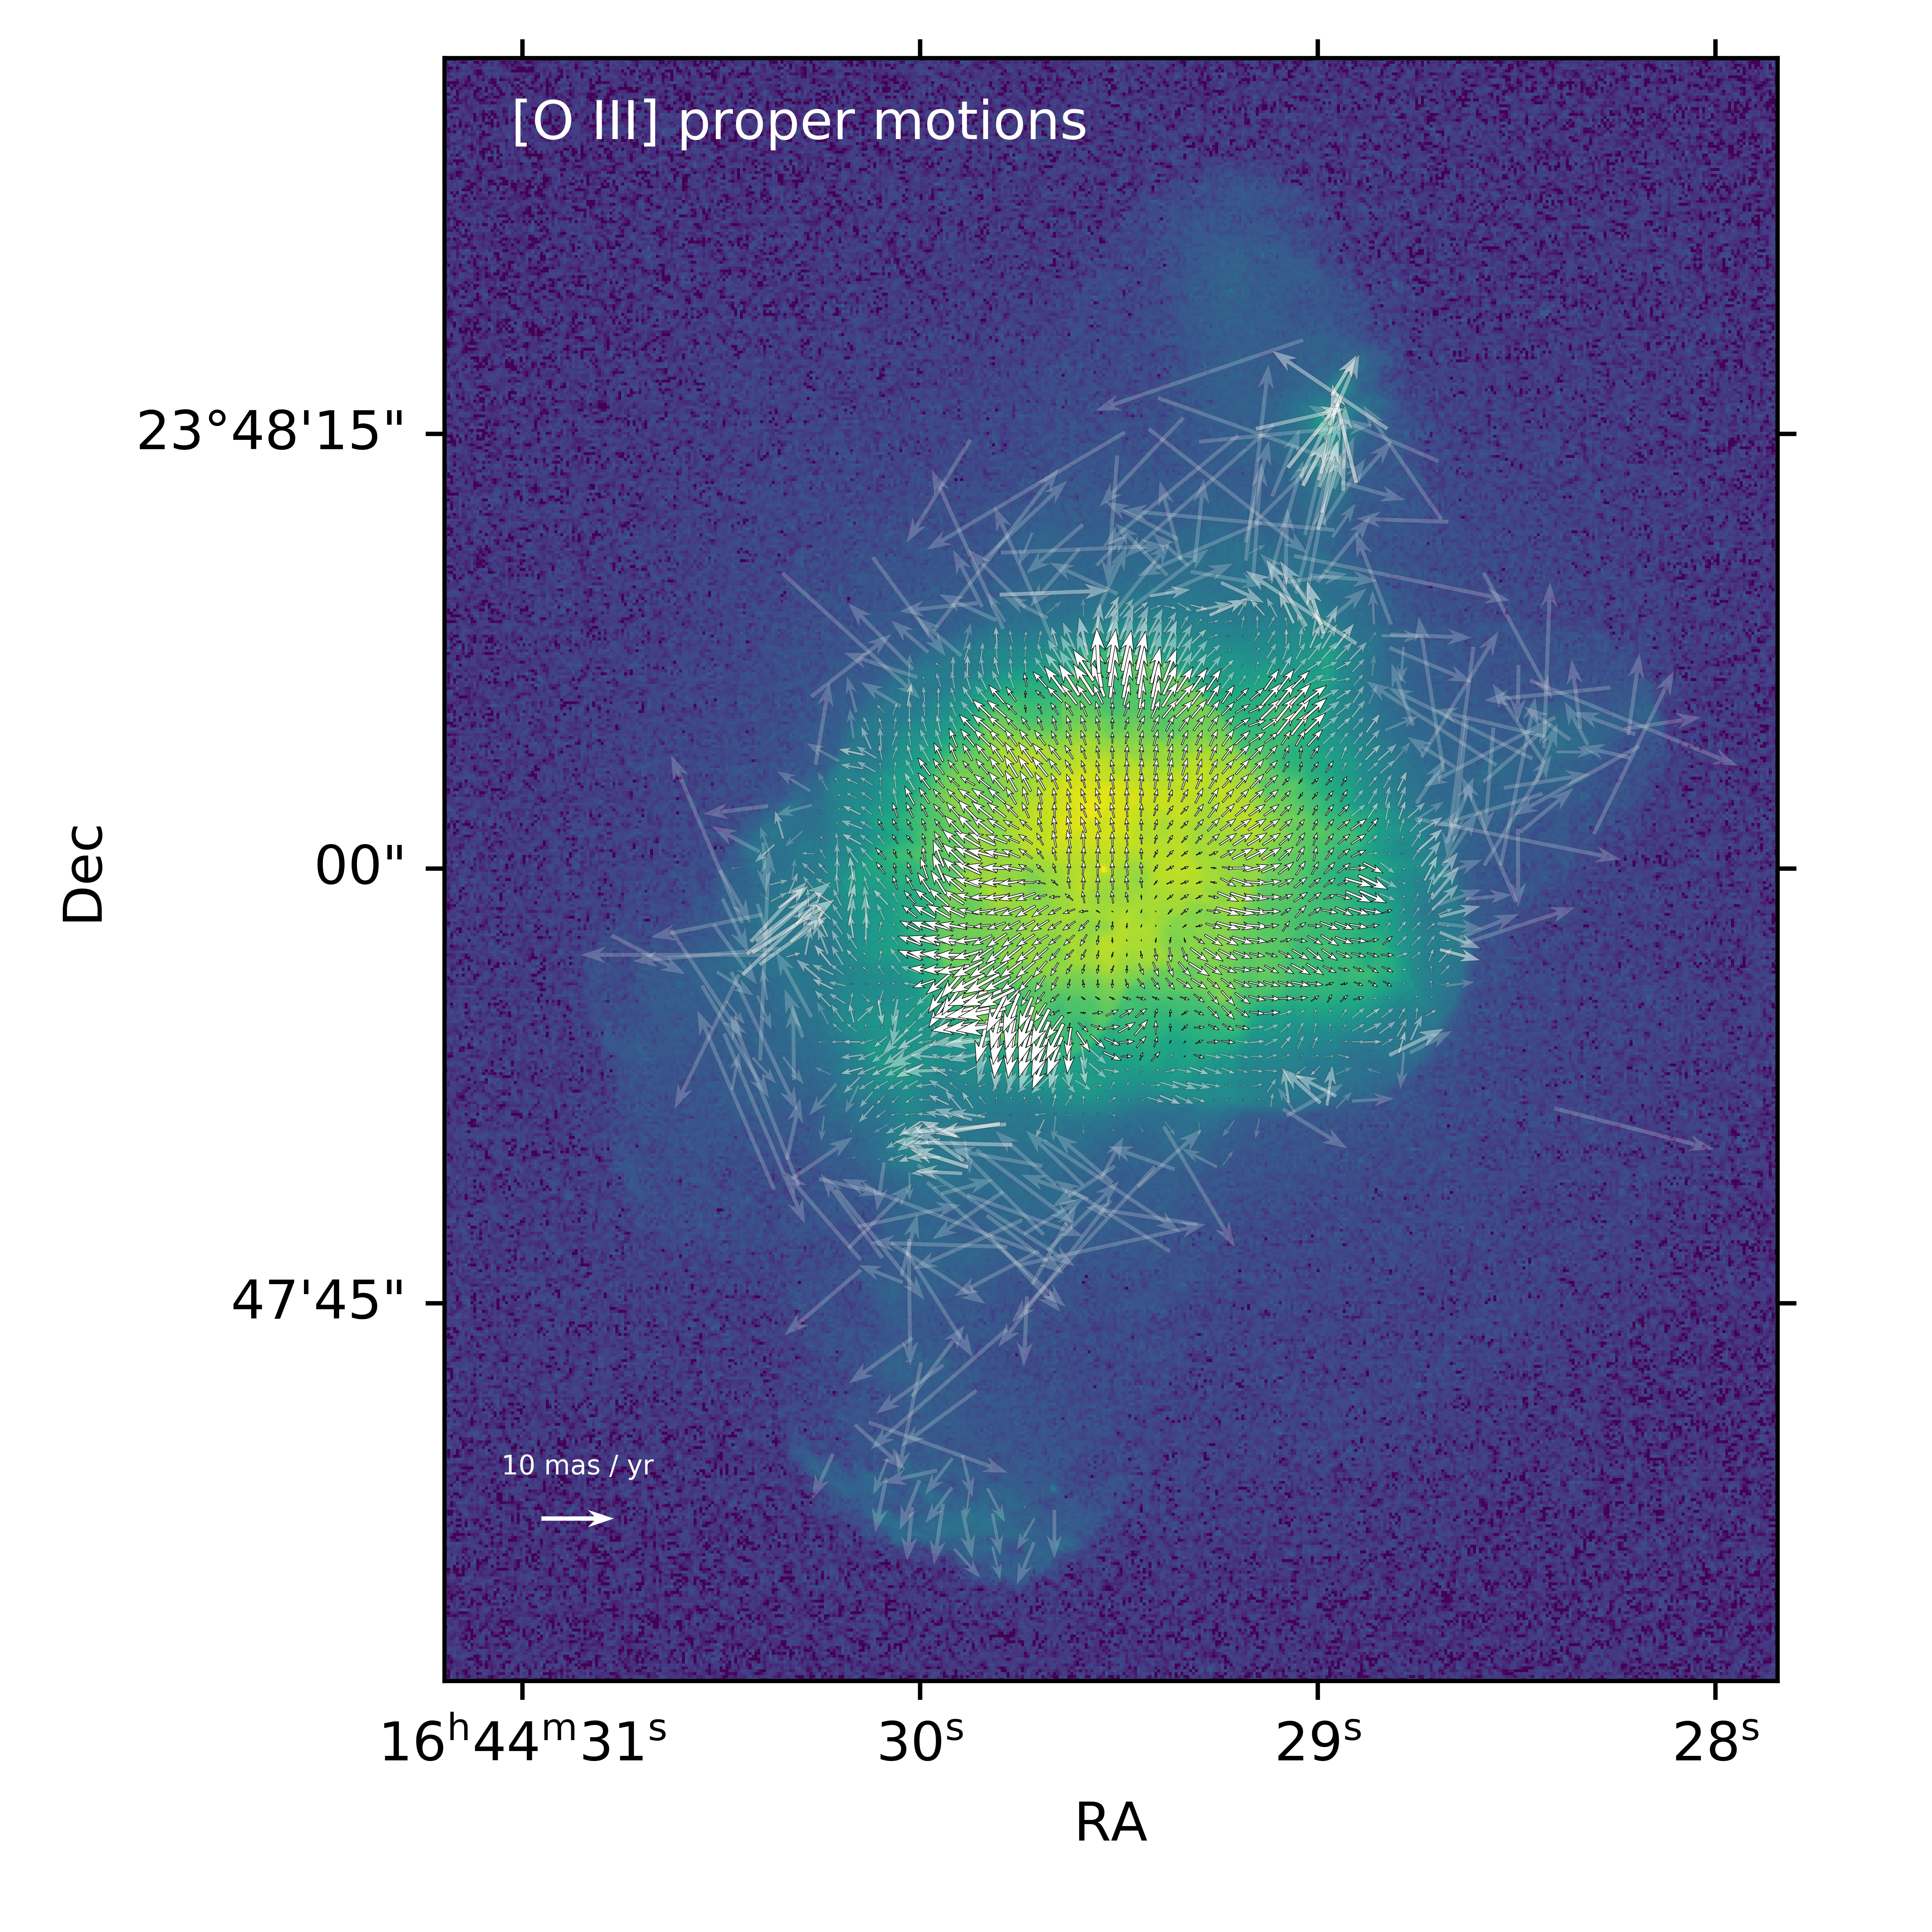
\includegraphics[width=\linewidth]{oiii-propermotions}
  \caption{Proper motions derived from two HST \oiii{} images (F502N
    filter) separated by 10.45 years, using the FLCT algorithm with a
    Gaussian window width of 10~pixels. The key at bottom left shows a
    proper motion of \SI{10}{mas.yr^{-1}}, corresponding to
    \SI{95}{km.s^{-1}} for an assumed distance of \SI{2}{kpc}.}
  \label{fig:proper-motions-oiii}
\end{figure}
\begin{figure}
  \centering
  \includegraphics[width=\linewidth]{nii-propermotions}
  \caption{As Fig.~\ref{fig:proper-motions-oiii} but for two HST
    \nii{} images (F658N filter). Note that the field of view is
    cropped slightly smaller than for \oiii{}.}
  \label{fig:proper-motions-nii}
\end{figure}

\section{Introduction}
\label{sec:introduction}

\section{Observations and data reduction}
\label{sec:observ-data-reduct}

\section{Longslit spectroscopy}
\label{sec:longsl-spectr}

\newpage
\section{Proper motions}
\label{sec:proper-motions}

Proper motions are calculated from HST WFPC2 imaging at two epochs separated by approximately 10 years,
using the FLCT method \citep{Welsch:2004a, Fisher:2008a}.\footnote{
  We used version 1.07 of FLCT, obtained from \url{http://cgem.ssl.berkeley.edu/cgi-bin/cgem/FLCT/home},
  together with version 1.04 of the Python wrapper pyflct,
  obtained from \url{https://github.com/PyDL/pyflct}.}
Results are shown in Figures~\ref{fig:proper-motions-oiii} and~\ref{fig:proper-motions-nii} for \oiii{} and \nii{}, respectively.
In both cases, the images were remapped to a uniform square pixel grid at the WFC resolution of \SI{0.1}{arcsec.pix^{-1}} before applying the algorithm.
The resultant per-pixel motions between the two epochs are found to be of order \SI{0.5}{pix} (\(\approx \SI{5}{mas.yr^{-1}}\))
and these raw results were then corrected by applying a global shift to force the motion of the central star to be zero.
The systematic error from the global alignment of the two epochs is estimated to be \SI{1.5}{mas.yr^{-1}},
which is expected to dominate the proper motion uncertainties in the brighter parts of the nebula.
In fainter and more featureless regions of the nebula, the proper motions are increasingly affected by random noise,
which can be seen in parts of the lobes in Figure~\ref{fig:proper-motions-oiii}.

The corrected results, as shown in the figures, can be seen to display motions that are predominantly radial from the central star.
To convert the angular motions into transverse velocities, we assume a distance of \SI{2}{kpc},
so that \SI{10}{mas.yr^{-1}} is equivalent to \SI{95}{km.s^{-1}}.
From the \oiii{} images (Fig.~\ref{fig:proper-motions-oiii}),
the fastest plane-of-sky motions are of order \SI{60}{km.s^{-1}},
and are chiefly along the NNW--SSE direction,
including the projected major axis of the inner peanut shell,
the NW~knot, the N~jet, and the end-cap of the S~lobe.
Motions along the perpendicular ENE--WSW direction are typically slower,
of order \SI{30}{km.s^{-1}}.
Note that proper motions are unavailable for the end cap of the N lobe since the second epoch HST image does not cover this region.

The \nii{} images (Fig.~\ref{fig:proper-motions-nii}) show a similar expansion pattern for the features that are visible in both lines.
Remarkably low plane-of-sky velocities of \(\le \SI{15}{km.s^{-1}}\) are seen for the \nii{}-bright knot complexes immediately north and west of the central star. 


\section{Kinematic components}
\label{sec:kinematic-components}

\subsection{Inner shells}
\label{sec:inner-shells}

\subsection{Knot complexes}
\label{sec:knot-complexes}

\subsection{Intermediate shell}
\label{sec:intermediate-shell}

\subsection{Outer lobes}
\label{sec:outer-lobes}

\subsection{Haloes}
\label{sec:haloes}

\section{Discussion}
\label{sec:discussion}

\subsection{Flow axes}
\label{sec:flow-axes}

\subsection{Dynamical ages}
\label{sec:dynamical-ages}

\bibliography{turtle-refs-will}


% Don't change these lines
\bsp	% typesetting comment
\label{lastpage}

\end{document}


%%% Local Variables:
%%% mode: latex
%%% TeX-master: t
%%% End:
